% ------------------------------------------------------------------------ %
% !TEX encoding = UTF-8
% !TEX TS-program = pdflatex
% !TEX root = ../Project.tex
% !TEX spellcheck = en-EN
% ------------------------------------------------------------------------ %
%
% ------------------------------------------------------------------------ %
% 	CHAPTER TITLE
% ------------------------------------------------------------------------ %
%
\chapter{Implementation, Integration and Test Plan}
%
\label{cap:implementationintegrationtestplan}
%
%
% ------------------------------------------------------------------------ %
%
\section{Implementation Order}
The implementation order of the tiers of the system is chosen in order to ease and speed up the integration of the complete system.
The first step is to have the database tier and then we can develop the business tier because it can be tested without any client but only by making API calls and it is requested to use the mobile application. The next thing to be developed is the mobile application or the web tier, but the decision was to develop the mobile application so that a client-server system is obtained. Then in order the web tier and the web browser will be implemented. 

\vspace{10mm}

\begin{center}
\thispagestyle{empty}
\makebox[\textwidth][c]{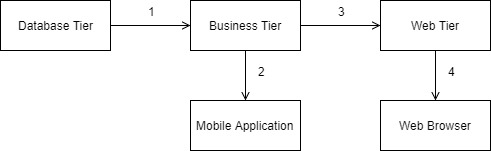
\includegraphics[width=1.2\textwidth]{MainMatter/images/it/imporder}}
\captionof{figure}{Implementation order of the system}
\end{center}
%
% ------------------------------------------------------------------------ %
%
\section{Integration and Test Plan}
This section describes the preparation of the integration testing activity for all the components, to reach the completed system.

\subsection{Entry criteria}
In order to enter in the integration testing phase some condition have to be satisfied, first thing RASD and DD of the system should be delivered. Furthermore, the development percentage of the components involved in the activity of integration has to be over a certain value (80\% for the components of this system) and the relative test units should be performed.

\subsection{Elements to Be Integrated} 
Referring to the section 2 -  Architectural design, the system can be divided in three categories of components: 
\begin{itemize}
\item	Front-end components: mobile application; 
\item	Back-end components: the server and its components;
\item	External components: the components which refer to functionalities provided by external systems and the DBMS.
\end{itemize} 
The front-end and the external components are independent one from each other, referring to back-end components some of them are not independent from others and need to be integrated. To fully integrate the three categories of components, some partial integration between categories need to be performed: front-end components and back-end components, and back-end components with external components.

\subsection{Integration Strategy}
The approach used for the integration testing phase is a bottom-up strategy, starting from components independent from other ones or components that depends only on one already developed. Then subsystem formed by the components tested, in turn, will be tested. This method will allow that a single component can be tested as soon as it’s finished (or almost completed), and so to parallelizeg the two phase of development and testing.


%
% -----------------------------END------------------------------------- %
